\subsection{Results on Stripe-82}
As discussed in Section~\ref{sec:runtime}, our approach has the potential 
to scale up to large astronomical surveys. We chose the image of M2 to test our method because ``ground truth" could be obtained from Hubble images to validate our results. Moreover, 
the PSF model is fairly realistic on M2: all sources are 
stars, and there are no galaxies in this region. 
However, most regions of the sky are much less 
crowded than M2.


We chose SDSS run 94, camcol 1, field  12 to examine our method on a sparse field more typical of SDSS 
images. After ten minutes of sleep training, we produced a catalog on the full $1489\times 2048$ image in $\approx2$ seconds (versus approximately six days of runtime for MCMC). 

This image is contained in Stripe 82, a region of the sky repeatedly imaged by SDSS. Averaging images from different runs boosts the signal to noise ratio and this {\itshape co-added} image can be analyzed to obtain a ground truth. 

However, this region of the sky also contains galaxies, which are 
not well-modelled by a PSF. A future paper will extend our generative model to include galaxies. For our setup, we trained Starnet using only the sleep phase (otherwise the model will try to use the PSF to explain both stars and galaxies in the wake-phase). 

Since this region of the sky is more sparse, we tile the image into $50\times 50$ tiles; $N_{max}$ on the tiles is three. 

Figure~\ref{fig:sparse_field} shows a $500\times 500$ subimage with 
our MAP catalog overlaid with the ground truth. We also report the 
TPR, comparing the stars in the co-added catalog with our estimated stars. (We have false defections, namely galaxies, and thus 
do not report the PPV). Of the stars in the co-added catalog with brightness at least $22.5$mag, we achieved a TPR of 90\%. 


\begin{figure}
    \centering
    \begin{subfigure}{0.45\textwidth}
        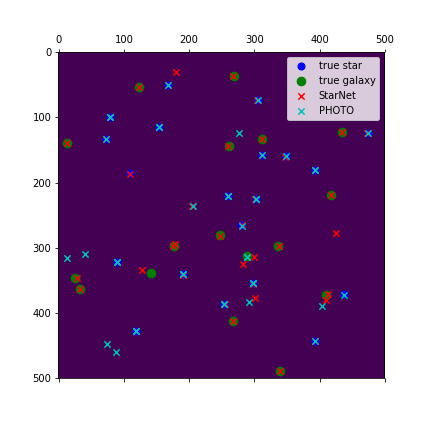
\includegraphics[width=\textwidth]{figures/sparse_field_detections.png}
        \label{fig:sparse_field_detect}
    \end{subfigure}
    \begin{subfigure}{0.54\textwidth}
        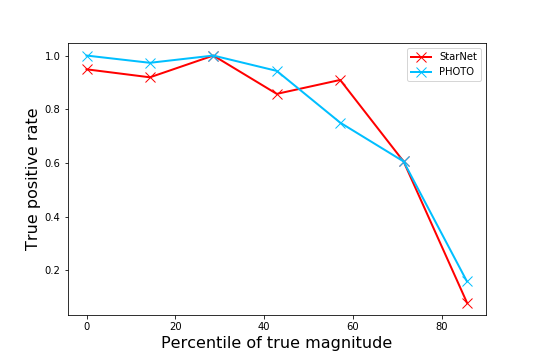
\includegraphics[width=\textwidth]{figures/sparse_field_tpr.png}
        \label{fig:sparse_field_tpr}
    \end{subfigure}
    \caption{(Left) a $500\times 500$ sparse field, with true stars in 
    blue, and true galaxies in green. Estimated stars are shown in red x's. 
    (Right) the true positive rate as a function of true magnitude. }
    \label{fig:sparse_field}
\end{figure}
